%%%%%%%%%%%%%%%%%%%%%%%%%%%%%%%%%%%%%%%%%%%%%%%%%%%%%%%%
%%%%%%%%%%%%%%%%%%%%%%%%%%%%%%%%%%%%%%%%%%%%%%%%%%%%%%%%
%%%%%%%%%%%%%%%%%%%%%%%%%%%%%%%%%%%%%%%%%%%%%%%%%%%%%%%%
\chapter{Optimization}
\label{chap:opt}
% TODO
% TODO many types of optimizers, two main classes of gradient and non-gradient methods.
% TODO A greedy optimizer finds the local optimum at each iteration, which may or may not converge to a global optimum.

%%%%%%%%%%%%%%%%%%%%%%%%%%%%%%%%%%%%%%%%%%%%%%%%%%%%%%%%
%%%%%%%%%%%%%%%%%%%%%%%%%%%%%%%%%%%%%%%%%%%%%%%%%%%%%%%%
\section{Maximum Likelihood Estimation (MLE)}
\label{opt:MLE}

Maximum likelihood estimation (MLE) is a method
of choosing the optimal parameters of a probability distribution
to match some set of observed data.
As the name suggests, MLE works by maximizing the likelihood of observing the given data.
Note that the terms likelihood and probability are closely related, but different, in this context.
Here probability refers to the probability of observing $x$ given parameters $\vb*{\beta}$, $P\left(x \mid \vb*{\beta}\right)$,
while likelihood refers to the likelihood of the distribution having parameters $\vb*{\beta}$ given an observation $x$, $L\left(\vb*{\beta} \mid x\right)$.
$L$ and $P$ are both equal to relevant probability distribution,
such as \cref{eq:stats:gaus:P} for the Gaussian distribution,
but which variables are independent and dependent changes.

As we wish to maximize the likelihood with respect to $\vb*{\beta}$,
we will be taking partial derivatives and finding where they equal zero, $\partial_{\vb*{\beta}} L = 0$.
In practice, likelihood functions are complicated\footnote{The value of $L$
is often close to $0$, making lack of precision an issue when doing computations.
$\log\left(L\right)$ is larger and also helps address this problem.} and
it is easier to maximize the log-likelihood $\log\left(L\right)$,
which has the same maximum as the original likelihood $L$,
but removes exponents and turns multiplication in to addition.
Generally there are $m$ points $\vb{x}_{i}$, each with $n$ dimensions, in a given dataset,
thus we are solving \cref{eq:MLE} for $\vb*{\beta} = \hat{\vb*{\beta}}_{\text{MLE}}$:

\begin{subequations}\label{eq:MLE}
\begin{align}
0 &= \partial_{\vb*{\beta}} \, L\left(\vb*{\beta} \mid \vb{x}\right) \label{eq:MLE:L} \\
\implies 0 &= \partial_{\vb*{\beta}} \log\left(L\left(\vb*{\beta} \mid \mathbf{X}\right)\right) = \partial_{\vb*{\beta}} \, \log\left(\prod_{i=1}^{m} \, P\left(\vb{x}_{i} \mid \vb*{\beta}\right)\right) \label{eq:MLE:log_L} \\
&= \sum_{i=1}^{m} \, \partial_{\vb*{\beta}} \log\left(P\left(\vb{x}_{i} \mid \vb*{\beta}\right)\right) \label{eq:MLE:log_L_sum}
\end{align}
\end{subequations}

In practice, it is unlikely that a closed form solution for $\hat{\vb*{\beta}}_{\text{MLE}}$ can be found
and numerical optimizers, such as gradient descent, are used instead.
Under certain conditions it can be shown that as $n \to \infty$ the MLE converges to $\hat{\vb*{\beta}}$,
\ie in the limit $n \to \infty$ no consistent estimator
has a lower MSE\footnote{More formally, the MLE achieves the Cram\'er--Rao lower bound.}.
Lastly, while the MLE is usually a biased estimator, see \cref{stats:bias},
the bias is also reduced as $n \to \infty$.

%%%%%%%%%%%%%%%%%%%%%%%%%%%%%%%%%%%%%%%%%%%%%%%%%%%%%%%%
\subsection{Exponential Distribution Example}
\label{opt:MLE:exp_ex}

We can use MLE to find the optimal $\hat{\lambda}_{\text{MLE}}$ of
the exponential distribution \cref{eq:stats:exp:P}
given a dataset of $m$ points, $x_{i}$, in 1 dimension:

\begin{subequations}\label{eq:MLE:exp_ex}
\begin{align}
0 &= \sum_{i=1}^{m} \partial_{\lambda} \log\left(P\left(x_{i} \mid \lambda\right)\right) = \sum_{i=1}^{m} \partial_{\lambda} \log\left(\lambda e^{-\lambda x_{i}}\right), \label{eq:MLE:exp_ex:log_L_sum} \\
&= \sum_{i=1}^{m}\partial_{\lambda} \left( \log\left(\lambda\right) -\lambda x_{i}\right) = \sum_{i=1}^{m} \frac{1}{\lambda} - x_{i} = \frac{m}{\lambda} - \sum_{i=1}^{m} x_{i}, \label{eq:MLE:exp_ex:solve} \\
\implies \hat{\lambda}_{\text{MLE}} &= \frac{m}{\sum_{i=1}^{m} x_{i}} = \frac{1}{\expval{x}}. \label{eq:MLE:exp_ex:lambda}
\end{align}
\end{subequations}

For another example of MLE see logistic regression \cref{eq:logistic:L_Pr}.

%%%%%%%%%%%%%%%%%%%%%%%%%%%%%%%%%%%%%%%%%%%%%%%%%%%%%%%%
%%%%%%%%%%%%%%%%%%%%%%%%%%%%%%%%%%%%%%%%%%%%%%%%%%%%%%%%
\section{Maximum A Posteriori (MAP)}
\label{opt:MAP}
% TODO In maximum \aposteriori (MAP) estimation
% TODO MLE is a special case of MAP with a uniform prior

%%%%%%%%%%%%%%%%%%%%%%%%%%%%%%%%%%%%%%%%%%%%%%%%%%%%%%%%
%%%%%%%%%%%%%%%%%%%%%%%%%%%%%%%%%%%%%%%%%%%%%%%%%%%%%%%%
\section{Gradient Descent}
\label{opt:grad_descent}
% TODO

%%%%%%%%%%%%%%%%%%%%%%%%%%%%%%%%%%%%%%%%%%%%%%%%%%%%%%%%
\subsection{Stochastic Gradient Descent (SGD)}
\label{opt:grad_descent:stochastic}
% TODO

%%%%%%%%%%%%%%%%%%%%%%%%%%%%%%%%%%%%%%%%%%%%%%%%%%%%%%%%
%%%%%%%%%%%%%%%%%%%%%%%%%%%%%%%%%%%%%%%%%%%%%%%%%%%%%%%%
\section{Lagrange Multipliers}
\label{opt:lagrange_mult}
% TODO

%%%%%%%%%%%%%%%%%%%%%%%%%%%%%%%%%%%%%%%%%%%%%%%%%%%%%%%%
%%%%%%%%%%%%%%%%%%%%%%%%%%%%%%%%%%%%%%%%%%%%%%%%%%%%%%%%
\section{Newton's Method}
\label{opt:newton}
% TODO

%%%%%%%%%%%%%%%%%%%%%%%%%%%%%%%%%%%%%%%%%%%%%%%%%%%%%%%%
%%%%%%%%%%%%%%%%%%%%%%%%%%%%%%%%%%%%%%%%%%%%%%%%%%%%%%%%
\section{Exploration-Exploitation Tradeoff}
\label{opt:EE_tradeoff}
% TODO

%%%%%%%%%%%%%%%%%%%%%%%%%%%%%%%%%%%%%%%%%%%%%%%%%%%%%%%%
%%%%%%%%%%%%%%%%%%%%%%%%%%%%%%%%%%%%%%%%%%%%%%%%%%%%%%%%
\section{Bayesian Bandits}
\label{opt:BB}
% TODO

%%%%%%%%%%%%%%%%%%%%%%%%%%%%%%%%%%%%%%%%%%%%%%%%%%%%%%%%
%%%%%%%%%%%%%%%%%%%%%%%%%%%%%%%%%%%%%%%%%%%%%%%%%%%%%%%%
\section{Evolutionary \& Genetic Algorithms}
\label{opt:evo}
% TODO

%%%%%%%%%%%%%%%%%%%%%%%%%%%%%%%%%%%%%%%%%%%%%%%%%%%%%%%%
%%%%%%%%%%%%%%%%%%%%%%%%%%%%%%%%%%%%%%%%%%%%%%%%%%%%%%%%
\section{Simulated Annealing}
\label{opt:SA}
% TODO

%%%%%%%%%%%%%%%%%%%%%%%%%%%%%%%%%%%%%%%%%%%%%%%%%%%%%%%%
%%%%%%%%%%%%%%%%%%%%%%%%%%%%%%%%%%%%%%%%%%%%%%%%%%%%%%%%
\section{Bayesian Optimization}
\label{opt:BO}

Frequently we are fortunate enough to have a fairly explicit form of
the objective function $S\left(\vb*{\beta}\right)$ to be optimized in order to solve a problem.
However, when $S\left(\vb*{\beta}\right)$ is not well-known,
is expensive to compute\footnote{The performance of a machine learning model as a function of its hyperparameters is a classic example of this.
In that case, evaluating $S$ amounts to training the model with a particular set of hyperparameters $\vb*{\beta}$,
then determining it's performance on a metric such as ROC AUC.}, or is non-differentiable,
the usual gradient based approaches, such as SGD and Newton's method, break down.
In these cases ``black box''\footnote{Black box as in
we do not have a closed-form expression for $S$, or know $\grad S$.} methods\footnote{Other examples of black box optimizers include
Tree-Structured Parzen Estimators (TPE),
genetic algorithms,
and some additional tree based methods described in \cite{Hutter2011,Hutter2014}.
A TPE is a close relative of Bayesian optimization, making use of the opposite side of Bayes' theorem by
estimating $P\left(\vb*{\beta} \mid S\right)$ and $P\left(S\right)$ rather than $P\left(S \mid \vb*{\beta}\right)$.
TPEs can accommodate categorical $\beta_{i}$ in a hierarchical manner,
however they can not model interactions between the $\beta_{i}$ \cite{bissuel_2019,NIPS2011_4443}.},
such as Bayesian optimization, may be used instead.

In Bayesian optimization\footnote{Generalized
formally as Sequential Model-Based Optimization (SMBO) \cite{NIPS2011_4443}.} \cite{Brochu2010,1301.1942,Borisyak,NIPS2011_4443},
$S$ is approximated by a well-known surrogate function\footnote{Also known as a response surface.}.
The surrogate typically is a Gaussian process (GP),
but can be any well-behaved regressor such as
a Random Forest or Boosted Decision Tree (BDT).
GPs \cref{eq:GP} are
extensions of Gaussian distributions which return a Gaussian at any point along their domain.
They are parameterized by a mean function\footnote{For convenience,
the prior $m\left(\vb{x}\right)$ is usually assumed to be zero, $m\left(\vb{x}\right)=0$.}, $m\left(\vb{x}\right)$,
and covariance function, $k\left(\vb{x}_{i}, \vb{x}_{j}\right)$,
\ie kernel\footnote{The kernel of the GP is a hyperparameter to be chosen in advance.
Standard kernel choices include
the radial basis function kernel $k\left(\vb{x}_{i}, \vb{x}_{j}\right) = \exp\left(-\frac{1}{2\sigma^{2}}\norm{\vb{x}_{i}-\vb{x}{j}}^{2}\right)$,
Mat\'{e}rn kernel,
and white noise kernel $k\left(\vb{x}_{i}, \vb{x}_{j}\right) \propto \delta_{ij}$.},
instead of a constant mean $\mu$ and variance $\sigma^{2}$.
An illustration of a GP is provided in \cref{fig:GP_ex}.

\begin{equation}\label{eq:GP}
f\left(\vb{x}\right) \sim \mathcal{GP}\left(m\left(\vb{x}\right), k\left(\vb{x}_{i}, \vb{x}_{j}\right)\right).
\end{equation}

\begin{figure}[H] % TODo might want to eventually remove
\centering
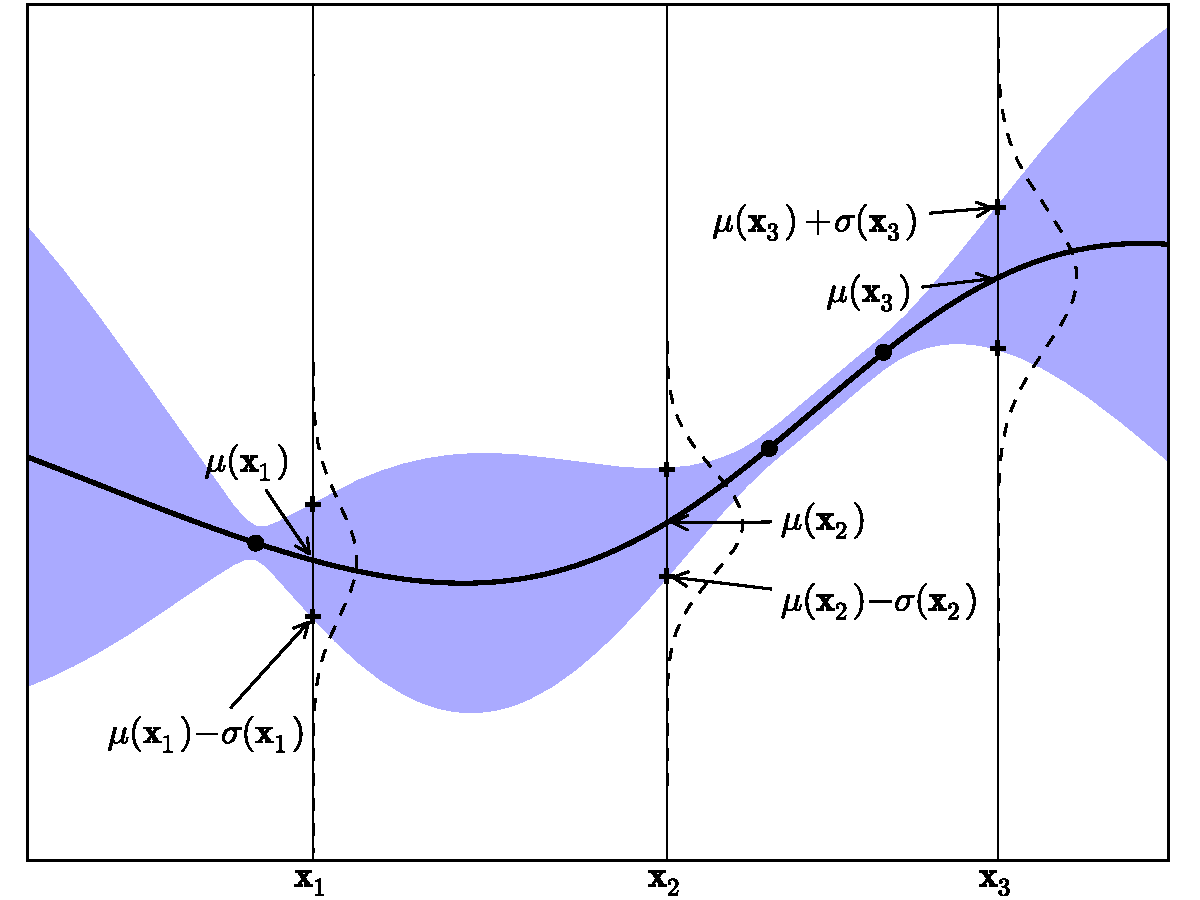
\includegraphics[width=0.85\textwidth]{figures/ml/gp}
\caption{
Illustration of a Gaussian process (GP) in 1D \cite{Brochu2010}.
Note that at any point $\vb{x}_{1}$, $\vb{x}_{2}$, $\vb{x}_{3}$ the GP
returns a Gaussian distribution characterizing the estimated mean and uncertainty on the
unknown true function, \ie the objective function $S\left(\vb*{\beta}\right)$ in the case of Bayesian optimization.
}
\label{fig:GP_ex}
\end{figure}

The surrogate function is initially fit to
a random sample of $\vb*{\beta}$, $S\left(\vb*{\beta}\right)$ points.
From this prior, Bayesian optimization
operates by iteratively sampling $S\left(\vb*{\beta}\right)$ and updating
the posterior surrogate function as each new piece of information is gained.
An acquisition function, $u\left(\cdot\right)$, directs the sampling,
estimating where $S\left(\vb*{\beta}\right)$ may be large
due to a high predicted value, large uncertainty, or some combination of the two.
The exploration-exploitation tradeoff inherent in $u\left(\cdot\right)$
can be tuned in various ways, see Section 2.3 of \cite{Brochu2010} for a full description\footnote{Common types of acquisition function include the
Expected Improvement (EI);
$\text{EI}\left(\vb*{\beta}\right) = \expvalE{\max\left(0,\,S\big(\vb*{\beta}\big) - S\big(\hat{\vb*{\beta}}\big)\right)}$
where $S\big(\hat{\vb*{\beta}}\big)$ is the current optimal value of $S$,
Upper Confidence Bound (UCB);
$\text{UCB}\left(\vb*{\beta}\right) = E_{\text{GP}} \left(\vb*{\beta}\right) + \kappa\,\text{var}_{\text{GP}} \left(\vb*{\beta}\right)$ where the mean and variance are of the GP and $\kappa$ sets the exploration-exploitation tradeoff,
and Maximum Probability of Improvement (MPI).}.
The iterative nature of Bayesian optimization is illustrated in \cref{fig:BO_ex}.
An accessible implementation of Bayesian optimization is available in \skopt \cite{scikit-optimize,Borisyak}.

\begin{figure}[H] % TODo might want to eventually remove
\centering
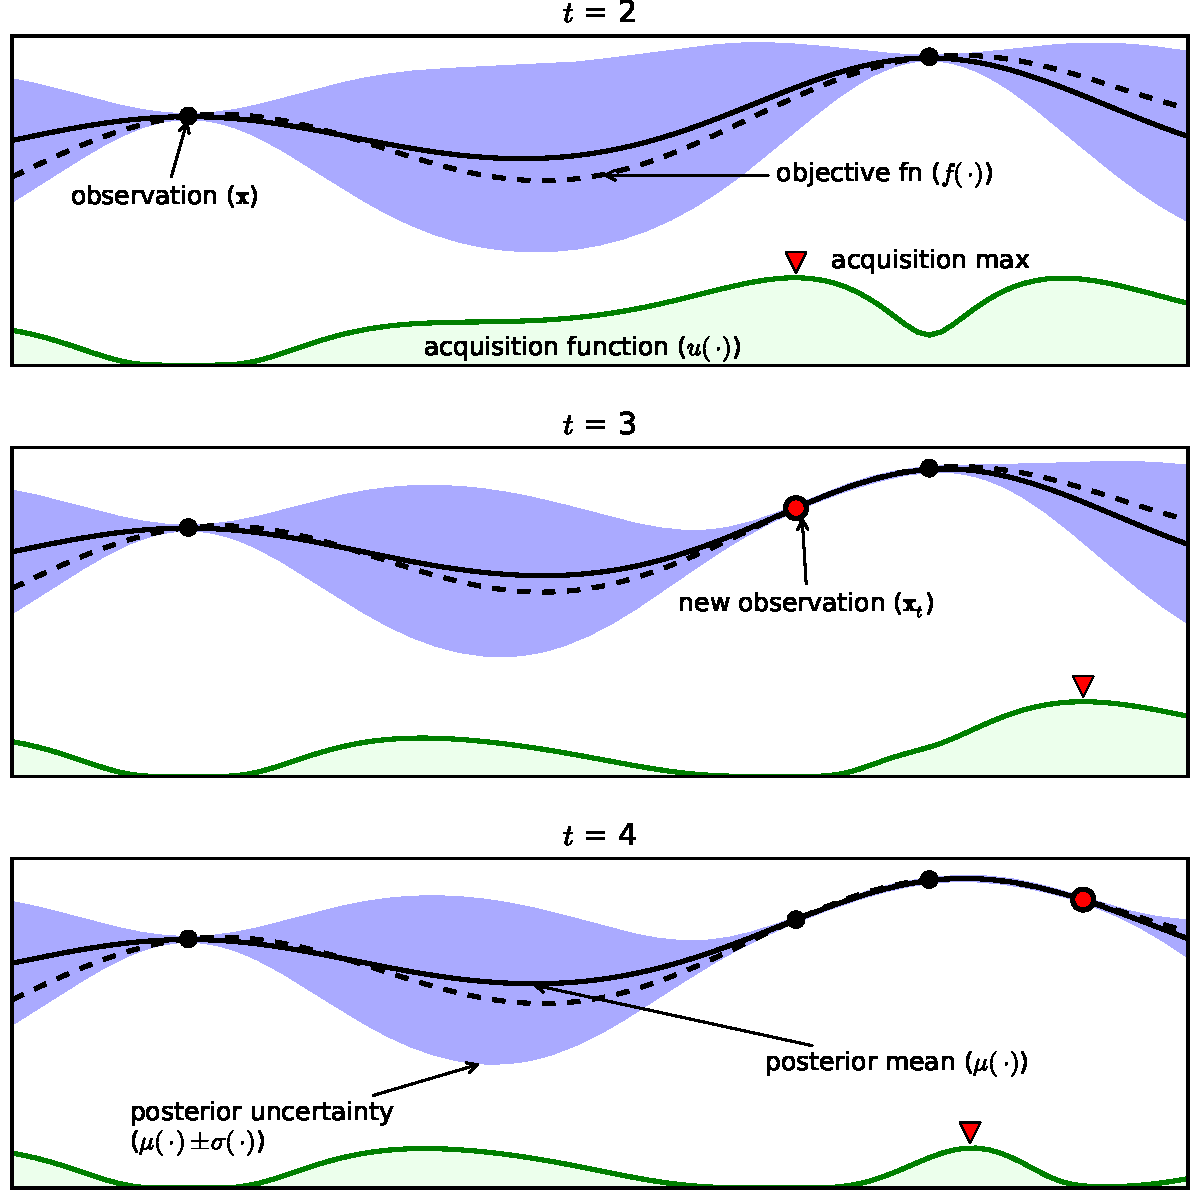
\includegraphics[width=0.85\textwidth]{figures/ml/toyGPtext3}
\caption{
Illustration of Bayesian optimization over three iterations in a toy 1D maximization problem \cite{Brochu2010}.
Note that the maximum of the acquisition function $u\left(\cdot\right)$
locates where $S\left(\vb*{\beta}\right)$ should be sampled next.
The GP estimated posterior distribution of $S\left(\vb*{\beta}\right)$
and $u\left(\cdot\right)$ are then updated.
This iterative process is repeated until the estimated maximum is satisfactory.
}
\label{fig:BO_ex}
\end{figure}

%%%%%%%%%%%%%%%%%%%%%%%%%%%%%%%%%%%%%%%%%%%%%%%%%%%%%%%%
%%%%%%%%%%%%%%%%%%%%%%%%%%%%%%%%%%%%%%%%%%%%%%%%%%%%%%%%
\section{Minimum Mean Square Error (MMSE) Estimator}
\label{opt:BO:MMSE}
% TODO
